\subsection{Bracketing Methods for Locating a Root}

\frame{
\frametitle{Consider a familiar topic of interest.}
Suppose that you save money by making regular monthly deposits $P$ and the annual interest rate is $I$; 
then the total amount $A$ after $N$ deposits is
\begin{equation*}
A = P + P(1+\frac{I}{12}) + P(1+\frac{I}{12})^2 + \cdots + P(1+\frac{I}{12})^{N-1}.
\end{equation*}
}

\frame{
\begin{itemize}
\item The first term on the right side of equation is the last payment. 
\item Then the next-to- last payment, which has earned one period of interest, contributes $P (1 + I /12)$. 
\item The second-from-last payment has earned two periods of interest and contributes $P (1 + I /12)^2$ , and so on. 
\item Finally, the last payment, which has earned interest for $N - 1$ periods, contributes $P (1 + I/12)^{N-1}$ toward the total. Recall that the formula for the sum of the $N$ terms of a geometric series is
\begin{equation*}
1 + r + r^2 + r^3 + \cdots + r^{N-1} = \frac{1-r^N}{1-r}
\end{equation*}
\end{itemize}
}

\frame{
We can write the amount $A$ equation  in the form
\begin{equation*}
A = P \left( 1+ (1 +\frac{I}{12}) + (1+\frac{I}{12})^2 + \cdots + (1+\frac{I}{12})^{N-1}  \right)
\end{equation*}
and use the substitution $r = (1 + I /12)$  to obtain
\begin{equation*}
A = P \frac{1 - \left(1 + \frac{I}{12}\right)^N}{1 - \left( 1 + \frac{I}{12} \right)}
\end{equation*}
This can be simplified to obtain the annuity-due equation,
\begin{equation*}
A = \frac{P}{\frac{I}{12}} \left( \left( 1 + \frac{I}{12} \right)^N - 1 \right)
\end{equation*}
}

\frame{
\begin{block}{Example.}
You save $\$250$ per month for $20$ years and desire that the total value of all payments and interest is $\$250, 000$ at the end of the $20$ years. What interest rate $I$ is needed to achieve your goal? 
\end{block}
If we hold $N = 240$ fixed, then $A$ is a function of $I$ alone; that is, $A = A(I)$. \\
We will start with two guesses, $I_0 = 0.12$ and $I_1 = 0.13$, and perform a sequence of calculations to narrow down the final answer. 
}

\frame{
Starting with $I_0 = 0.12$ yields
\begin{equation*}
A(0.12) = \frac{250}{0.12/12} \left( \left( 1 + \frac{0.12}{12} \right)^240 - 1\right) = 247,314
\end{equation*}
Since this value is a little short of the goal, we next try $I_1 = 0.13$:
\begin{equation*}
A(0.13) = \frac{250}{0.13/12} \left( \left( 1 + \frac{0.13}{12} \right)^240 - 1\right) = 282,311
\end{equation*}
This is a little high, so we try the value in the middle $I_2 = 0.125$:
\begin{equation*}
A(0.125) = \frac{250}{0.125/12} \left( \left( 1 + \frac{0.125}{12} \right)^240 - 1\right) = 264,623
\end{equation*}
}

\frame{
This is again high and we conclude that the desired rate lies in the interval $[0.12, 0.125]$. \\
The next guess is the midpoint $I_3 = 0.1225$:
\begin{equation*}
A(0.1225) = \frac{250}{0.1225/12} \left( \left( 1 + \frac{0.1225}{12} \right)^240 - 1\right) = 255,803
\end{equation*}
This is high and the interval is now narrowed to $[0.12, 0.1225]$. 
Our last calculation uses the midpoint approximation $I_4 = 0.12125$:
\begin{equation*}
A(0.12125) = \frac{250}{0.12125/12} \left( \left( 1 + \frac{0.12125}{12} \right)^240 - 1\right) = 251,518
\end{equation*}
}

\frame{
\begin{itemize}
\item Further iterations can be done to obtain as many significant digits as required.
\item The purpose of this example was to find the value of $I$ that produced a specified level $L$ of the function value, that is, to find a solution to $A(I) = L$. 
\item It is standard practice to place the constant $L$ on the left and solve the equation $A(I) - L = 0$.
\end{itemize}
}

\frame{
\begin{block}{Definition.}
Assume that $f (x)$ is a continuous function. Any number $r$ for which $f (r) = 0$ is called a {\Large root of the equation} $f (x) = 0$. 
Also, we say that $r$ is a {\Large zero of the function} f (x).
\end{block}
\vspace{0.5cm}
For example,\\
the equation $2x^2 + 5x - 3 = 0$ has two real roots $r_1 = 0.5$ and $r_2 = -3$, 
whereas the corresponding function $f (x) = 2x^2 +5x -3 = (2x -1)(x +3)$ has two real zeros, $r_1 = 0.5$ and $r_2 = -3$.
}

\frame{
\frametitle{Bisection Method of Bolzano}
\framesubtitle{The bracketing method for finding a zero of a continuous function}
\begin{itemize}
\item We must start with an initial interval $[a, b]$, where $f (a)$ and $f (b)$ have opposite signs. 
\vspace{0.3cm}
\item Since the graph $y = f (x)$ of a continuous function is unbroken, it will cross the $x -$ axis at a zero $x = r$ that lies somewhere in the interval. 
\vspace{0.3cm}
\item The bisection method systematically moves the endpoints of the interval closer and closer together until we obtain an interval of arbitrarily small width that brackets the zero.
\end{itemize}
}

\frame{
\begin{block}{The decision step for this process of interval halving is first to choose the midpoint $c = (a + b)/2$ and then to analyze the three possibilities that might arise:}
\begin{itemize}
\item If $f (a)$ and $f (c)$ have opposite signs, a zero lies in $[a, c]$. 
\item If $f (c)$ and $f (b)$ have opposite signs, a zero lies in $[c, b]$.
\item If $f(c) = 0$, then the zero is $c$.
\end{itemize}
\end{block}
\begin{columns}
\begin{column}{0.5\textwidth}
\begin{figure}
\begin{center}
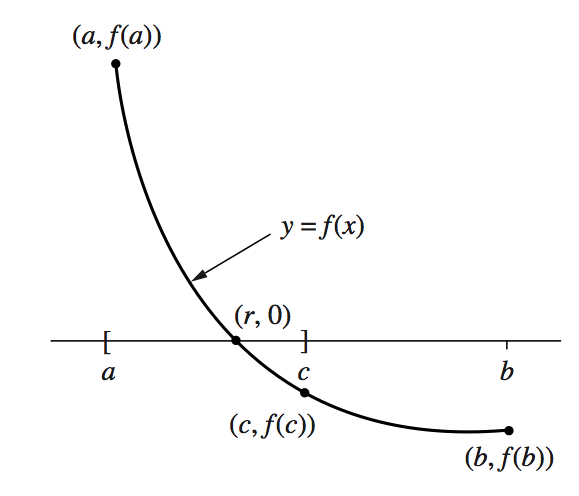
\includegraphics[width=50mm]{chap-1/fig_2-6.png}
\caption{If $f(a)$ and $f(c)$ have opposeite signs, then squeeze from the right.}
\end{center}
\end{figure}
\end{column}
\begin{column}{0.5\textwidth}
\begin{figure}
\begin{center}
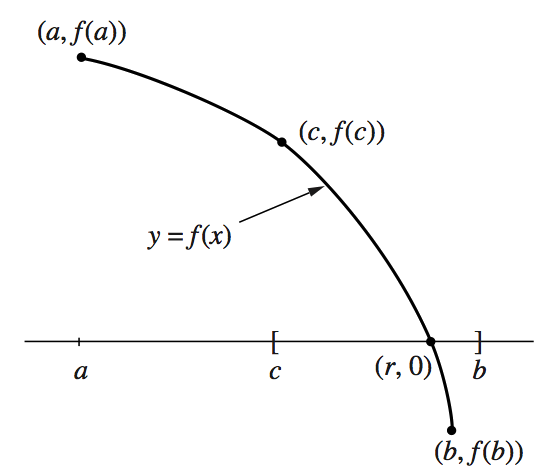
\includegraphics[width=50mm]{chap-1/fig_2-6_2.png}
\caption{If $f(c)$ and $f(b)$ have opposite signs, then squeeze from the left.}
\end{center}
\end{figure}
\end{column}
\end{columns}
}

\frame{
\begin{block}{Theorem (Bisection Theorem).}
Assume that $f \in C[a, b]$ and that there exists a number $r \in [a,b]$ such that $f(r) = 0$. 
If $f(a)$ and $f(b)$ have opposite signs, and $\{c_n\}_{n=0}^{\infty}$ represents the sequence of midpoints generated by the bisection process, then
\begin{equation*}
\left| r-c_n \right| \le \frac{b-a}{2^{n+1}} \ \ \ for n=0, 1, \ldots, 
\end{equation*}
and therefore the sequence $\{c_n\}_{n=0}^{\infty}$ converges to the zero $x = r$;
that is,
\begin{equation*}
\lim_{n \rightarrow \infty} c_n = r. 
\end{equation*}
\end{block}
}

\frame{
\frametitle{Proof of Theorem.}
Since both the zero $r$ and the midpoint $c_n$ lie in the interval $[a_n , b_n ]$, the distance between $c_n$ and $r$ cannot be greater than half the width of this interval. 
Thus
\begin{equation*}
\left| r - c_n \right| \le \frac{b_n-a_n}{2} \ \ \ for \  all \ n.
\end{equation*}
Observe that the successive interval widths form the pattern
\begin{equation*}
\begin{array}{l}
b_1 - a_1 = \frac{b_0 - a_0}{2^1} \\
b_2 - a_2 =\frac{b_1-a_1}{2} = \frac{b_0 - a_0}{2^2}. \\
\end{array} 
\end{equation*}
}

\frame{
\begin{equation*}
\begin{array}{c}
b_n - a_n = \frac{b_0 - a_0}{2^{n+1}}. \\
\Downarrow \\
|r-c_n| \le \frac{b_0 - a_0}{2^{n+1}} \ \ \ for \ all \ n.
\end{array}
\end{equation*}
\begin{figure}
\begin{center}
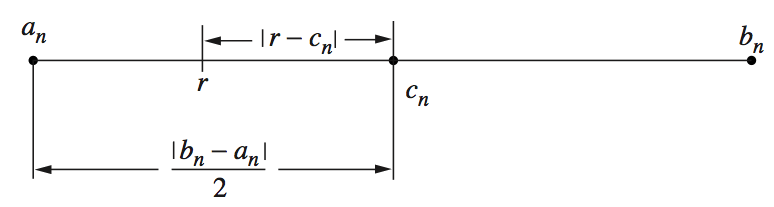
\includegraphics[width=100mm]{chap-1/fig_2-7.png}
\caption{The root $r$ and midpoint $c_n$ of $[a_n,b_n]$ for the bisection method.}
\end{center}
\end{figure}
}

\frame{
\begin{block}{Example.}
The function $h(x) = x \sin(x)$ occurs in the study of undamped forced oscillations. 
Find the value of $x$ that lies in the interval $[0, 2]$, where the function takes on the value $h(x) = 1$ (the function sin(x) is evaluated in radians).
\end{block}
We use the bisection method to find a zero of the function $f (x) = x \sin(x) - 1$. 
Starting with $a_0 = 0$ and $b_0 =2$, we compute
\begin{equation*} 
f (0) = -1.000000 \ \ \ and \ \ \ f (2) = 0.818595, 
\end{equation*}
so a root of $f(x) = 0$ lies in the interval $[0,2]$. 
At the midpoint $c_0 = 1$, we find that $f (1) = -0.158529$. 
Hence the function changes sign on $[c_0, b_0] = [1, 2]$.
}

\frame{
\begin{figure}
\begin{center}
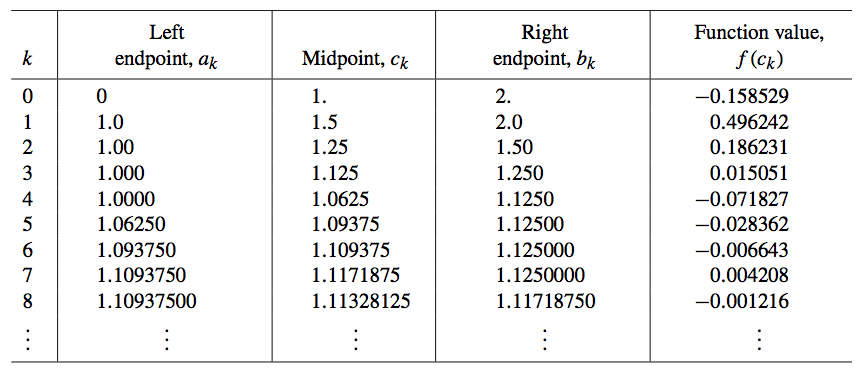
\includegraphics[width=90mm]{chap-1/tab_2-1.png}
\end{center}
\end{figure}
In this manner we obtain a sequence $\{c_k\}$ that converges to $r \approx 1.114157141$.
}

\frame{
\frametitle{Method of {\huge false position} or the {\huge regula false} method}
\framesubtitle{It was developed because the bisection method converges at a fairly slow speed.}
We assume that $f (a)$ and $f (b)$ have opposite signs. 
A better approximation is obtained if we find the point $(c, 0)$ where the secant line $L$ joining the points $(a, f (a))$ and $(b, f (b))$ crosses the x-axis. 
\begin{columns}
\begin{column}{0.5\textwidth}
\begin{figure}
\begin{center}
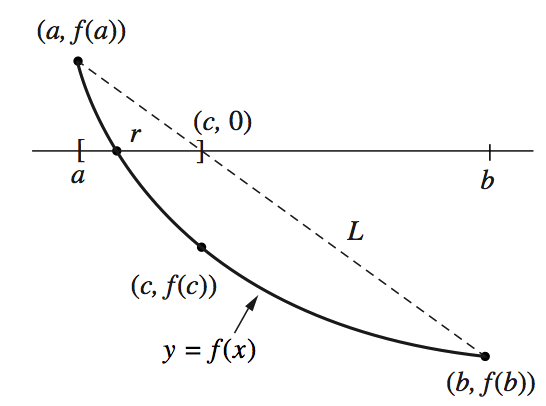
\includegraphics[width=45mm]{chap-1/fig_2-8.png}
\caption{If $f(a)$ and $f(c)$ have opposeite signs, then squeeze from the right.}
\end{center}
\end{figure}
\end{column}
\begin{column}{0.5\textwidth}
\begin{figure}
\begin{center}
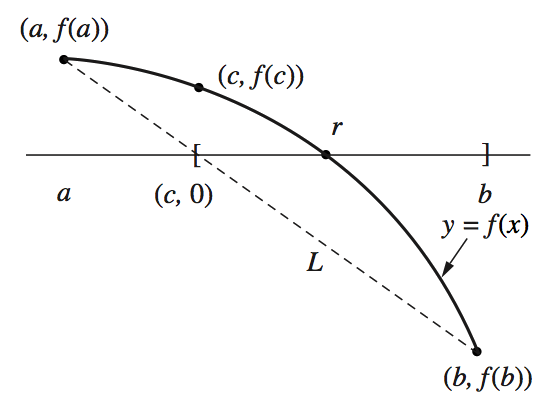
\includegraphics[width=45mm]{chap-1/fig_2-8_2.png}
\caption{If $f(c)$ and $f(b)$ have opposite signs, then squeeze from the left.}
\end{center}
\end{figure}
\end{column}
\end{columns}
}

\frame{
To find the value $c$, we write down two versions of the slope m of the line $L$:
\begin{equation*}
m = \frac{f(b)-f(a)}{b-a}
\end{equation*}
where the points $(a, f (a))$ and $(b, f (b))$ are used, and 
\begin{equation*}
m = \frac{0- f(b)}{c-b}
\end{equation*}
the points $(c, 0)$ and $(b, f (b))$ are used.
}

\frame{
We can get :
\begin{equation*}
\frac{f(b)- f(a)}{b-a} = \frac{0- f(b)}{c-b}
\end{equation*}
which is easily solved for $c$ to get 
\begin{equation*}
c = b- \frac{f(b)(b-a)}{f(b)- f(a)}
\end{equation*}
\begin{block}{The three possibilities are the same as before:}
\begin{itemize}
\item If $f (a)$ and $f (c)$ have opposite signs, a zero lies in $[a, c]$. 	
\item If $f (c)$ and $f (b)$ have opposite signs, a zero lies in $[c, b]$.
\item If $f(c)=0$,then the zero is c.
\end{itemize}
\end{block}
}


\frame{
\frametitle{Exercises and Program}
\begin{block}{}
Find an approximation for the interest rate $I$ that will yield the total annuity value $A$ if $240$ monthly payments $P$ are made.  \\
Use the two starting values for $I$ and compute the next three approximations using the bisection method.
\begin{itemize}
\item $P = \$275$, $A = \$250,000$, $I_0 = 0.11$, $I_1 = 0.12$
\item $P = \$325$, $A = \$400,000$, $I_0 = 0.13$, $I_1 = 0.14$
\end{itemize}
\end{block}
}

